
\documentclass[12pt]{article}
\usepackage{geometry}
 \geometry{letterpaper,left=25mm,top=25mm,right=25mm}
\usepackage[utf8]{inputenc}
\usepackage[spanish]{babel} %Poner algunas palabras reservadas en español
\usepackage{authblk} %Poner instituto en la portada
%Paquetes para símbolos matematicos
\usepackage{amsmath}
\usepackage{mathtools}
\usepackage{amsthm}
\usepackage{amssymb}
\usepackage{bbm}
\usepackage[]{algorithm2e} %Paquete para algoritmos
\usepackage{enumerate}
%Paquete para imagenes
\usepackage{graphicx}
\graphicspath{{img/}}
%Paquete para teoremas
\newtheorem*{thm}{Teorema}
%Quitar la sangria
\setlength{\parindent}{0cm}

\title{Tarea 2}
\author{Fernando Márquez Pérez \\ Juan Antonio Jasso Oviedo \\ Emiliano Dom\'inguez Cruz}
\date{04/10/2019}
\affil{Facultad de Ciencias\\UNAM}

\begin{document}
\begin{titlepage}
    \maketitle
\end{titlepage}

%EJERCICIO 1 ----------------------------------------------------------------------------------
1. Determine si las siguientes funciones son continuas en \(x_0\).

\begin{enumerate}[\hspace{9px} a)]
    \item
    \( f(x)=
    \begin{cases}
        \sqrt{x^2-1}\text{, si} \ x \geq 1\\
        x^2-2x+1\text{, si} \ x \in [0,1]
    \end{cases}
    \)
    en $x_0 = 1$\\
    \item
    \( h(x)=
    \begin{cases}
        \frac{|x|}{x}\text{, si} \ x \neq 0\\
        1\text{, si} \ x=0\\
    \end{cases}
    \)
    en $x_0=0$
    \item
    \( g(x)=
    \begin{cases}
        \sqrt{1-x^2}\text{, si} \ x \in [0,1]\\
        -\sqrt{1-(x-2)^2}\text{, si} \ x \in [1,2]
    \end{cases}
    \)
    en $x_0=1$
\end{enumerate}

%EJERCICIO 2 ----------------------------------------------------------------------------------
2. Se inyecta un fármaco a un paciente cada 12 horas. En la Fig. 1 se muestra la concentración $c(t)$ del fármaco en el torrente sanguieo después de $t$ horas.
\begin{figure}[h]
    \centering
    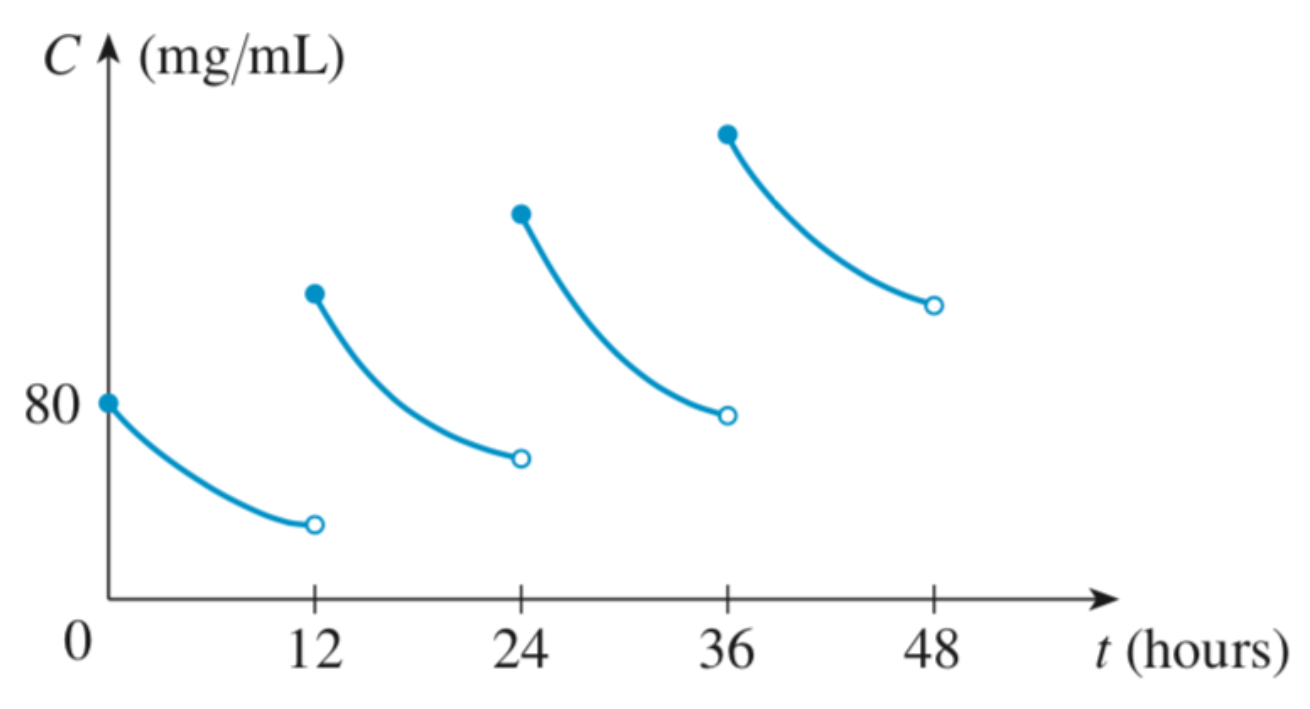
\includegraphics[width=0.5\textwidth]{fig1}
    \caption{Concentraci\'on de f\'armaco}
    %Para referenciarla usar \ref{fig1}
    \label{fig1}
\end{figure}
\begin{enumerate}[\hspace{9px} a)]
    \item ¿Para qué valores de $t$, $c(t)$ tiene discontinuidades?
    \item ¿Qué tipo de discontinuidades tiene?
\end{enumerate}

%EJERCICIO 3 ----------------------------------------------------------------------------------
3. Mostrar que existe algún número $x$, tal que:

\begin{enumerate}[\hspace{9px} a)]
    %EJERCICIO A
    \item \(\sin x = x-1\)\\

        Reescribimos la igualdad como \(\sin(x)-(x-1)=0 \Longrightarrow \sin(x)-x+1=0\)\\

        Como $\sin(x)$ es continua y $x-1$ es un polinomio y todos los polimonios son continuos. Su suma es una función continua. Entonces \(f(x)=\sin(x)-x+1\) es continua en todos los $\mathbbm{R}$.\\

        Para utilizar el TVI, buscamos $f(a)$ y $f(b)$ tal que $f(a)<0<f(b)$.\\

        Proponemos $a=0$ y $b=\pi$
        \[f(0)=\sin(0)-0+1=0-0+1=1\]
        \[f(\pi)=\sin(\pi)-\pi+1=0-\pi+1 \approx -2.1416\]

        Como $f$ es continua en el intervalo $[0,\pi]$ y \(f(0)>0>f(\pi)\), podemos utilizar un derivado del TVI (Parte de un corolario) para decir que: \[\exists \ x_0 \in (0,\pi) : \ f(x_0)=0\]

    %EJERCICIO B
    \item \(x^{179}+\displaystyle\frac{163}{1+x^2+\sin^2 x}=119\)\\

        Reescribimos la igualdad como \(x^{179}+\displaystyle\frac{163}{1+x^2+\sin^2 x}-119=0\)\\

        Como $\sin(x)$ es continua, $\sin^2(x)$ es continua. De igual manera, $x^2$ es continua, por lo que $1+x^2+\sin^2(x)$ es continua.

        \[0<1<1+x^2+\sin^2(x) \quad \text{Porque, por el cuadrado, ambos son positivos $\forall \ x \in \mathbbm{R}$}\]

        Como $1+x^2+\sin^2(x)$ nunca es 0, $\displaystyle\frac{163}{1+x^2+\sin^2(x)}$ es continua en todos los $\mathbbm{R}$. $x^{179}$ también es continua, por lo que \(f(x)=x^{179}+\displaystyle\frac{163}{1+x^2+\sin^2(x)}-119\) \ es continua en todos los $\mathbbm{R}$.\\

        Para utilizar el TVI, buscamos $f(a)$ y $f(b)$ tal que $f(a)<0<f(b)$.\\

        Proponemos $a=-1$ y $b=0$
        \[f(0)=0^{179}+\displaystyle\frac{163}{1+0^2+\sin^2(0)}-119 = 0+\displaystyle\frac{163}{1+0+0}-119 = 163-119 = 44\]
        \begin{multline*}
            f(-1)=(-1)^{179}+\displaystyle\frac{163}{1+(-1)^2+\sin^2(-1)}-119 \approx -1+\displaystyle\frac{163}{1+1+1}-119 \\ \approx -1+\displaystyle\frac{163}{3}-119 \approx -1+54.3-119 \approx -65.7
        \end{multline*}

        Nota: La respuesta correcta es $f(-1)=-59.8$, y difiere de lo obtenido por que $\sin(-1)=-0.84$ y nosotros consideramos $\sin(-1) \approx -1$\\

        Como $f$ es continua en el intervalo $[-1,0]$ y \(f(-1)<0<f(0)\), podemos utilizar el TVI para decir que: \[\exists \ x_0 \in (-1,0) : \ f(x_0)=0\]

    %EJERCICIO C
    \item \(\cos x - \displaystyle\frac{1}{2}=x-1\)\\

        Reescribimos la igualdad como \(\cos(x)-\displaystyle\frac{1}{2}-(x-1)=0 \Longrightarrow \cos(x)+\displaystyle\frac{1}{2}-x=0\).\\

        Como $\cos(x)$ y $x$ son continuos, y la suma de continuos es continua, $f(x)=\cos(x)-x+\displaystyle\frac{1}{2}$ es continua en todos los $\mathbbm{R}$.\\

        Para utilizar el TVI, buscamos $f(a)$ y $f(b)$ tal que $f(a)<0<f(b)$.\\

        Proponemos $a=0$ y $b=\pi$
        \[f(0)=\cos(0)-0+\frac{1}{2} = 1-0+\frac{1}{2} = \frac{3}{2}\]
        \[f(\pi)=\cos(x)-x+\frac{1}{2} = 0-\pi+\frac{1}{2} \approx -2.6\]

        Como $f$ es continua en el intervalo $[0,\pi]$ y \(f(0)>0>f(\pi)\), podemos utilizar un derivado del TVI (Parte de un corolario) para decir que: \[\exists \ x_0 \in (0,\pi) : \ f(x_0)=0\]

    %EJERCICIO D
    \item \((2x^2-2)^2=-x+1\)\\

    Reescribimos la igualdad como \((2x^2-2)^2-(-x+1)=0 \Longrightarrow (2x^2-2)^2+x-1=0\).\\

    Como $2x^2-2$ y $-x+1$ son polinomios, son continuos. Como la multiplicación de dos continuos es continua, $(2x^2-2)^2$ es continua. Y dado que la suma de dos continuos es continua $f(x)=(2x^2-2)^2+x-1$ es continua en todos los $\mathbbm{R}$.\\

    Para que $f$ cumpla el TVI tiene que existir un $f(x_0)<0$, pero $f$ nunca es menor a 0:

    Observación: Sabemos que $(2x^2-2)^2 \geq 0 \ \forall \ x \in \mathbbm{R}$\\

    Para $x \leq 1$:
    \[x \leq 1 \Rightarrow x-1 \leq 0 \leq (2x^2-2)^2 \Rightarrow x-1 \leq (2x^2-2)^2 \Rightarrow 0 \leq (2x^2-2)^2-(x-1)\]

    Para $x>1$:
    \[x>1 \Rightarrow x-1>0 \Rightarrow x-1+(2x^2-2)^2>0\]

    Pero si proponemos $x_0=1$:

    \[f(1)=(2(1)^2-2)^2+1-1=(2-2)^2+0=0^2+0=0\]

    Obtenemos el $x_0$ que cumple la igualdad.\\

\end{enumerate}

%EJERCICIO 4 ----------------------------------------------------------------------------------
4. Vea si en los siguientes incisos se cumple el teorema de valor intermedio y, en ese caso, calcula un valor intermedio.

\begin{enumerate}[\hspace{9px} a)]
    %EJERCICIO A
    \item \(f(x)=x^3\) en $[-1,1]$\\

        Obtenemos $f(-1)$ y $f(1)$:
        \begin{align*}
            &f(-1) = (-1)^3 = -1  &&f(1) = (1)^3 = 1
        \end{align*}

        Sabemos que $f$ es un polinomio de grado 3 y que todos los polinomios son continuos en $\mathbbm{R}$, por ende, $f$ es continua en $[-1,1]$.\\

        Como $f(-1) < 0 < f(1)$ y $f(x)$ es continua en $[-1,1]$. Podemos usar el \textbf{Teorema del Valor Intermedio} para decir que: \(\exists \ x_0 \in (-1,1) : \ f(x_0)=0\).\\

        Ahora buscamos a $x_0$:
        \begin{equation*}
            f(x_0)=0 \Rightarrow (x_0)^3 = 0 \Rightarrow (x_0)(x_0)(x_0)=0 \Rightarrow x_0=0
        \end{equation*}

        \textbf{$\mathbf{\therefore \ f(x)}$ cumple el Teorema del Valor Intermedio en el intervalo dado. Un valor intermedio es $\mathbf{x_0=0}$.}\\

    %EJERCICIO B
    \item \(g(x)=x^3\) en $[0,2]$\\

        Obtenemos $g(0)$ y $g(2)$:
        \begin{align*}
            &g(0)=(0)^3=0 &&g(2)=(2)^3=8
        \end{align*}

        Estrictamente hablando, $g(x)$ no cumple el \textbf{Teorema del Valor Intermedio} porque \(g(0) < 0 < g(2)\) no es verdad porque $g(0)=0$. Pero es eso se debe a que justo el intervalo toma al $x_0$ que cumple $g(x_0)=0$: $\mathbf{x_0=0}$\\

    %EJERCICIO C
    \item \(h(x)=x^2+4x+4\) en $[0,1]$\\

        Obtenemos $h(0)$ y $h(1)$:
        \begin{align*}
            &h(0)=(0)^2+4(0)+4=4 &&h(1)=(1)^2+4(1)+4=1+4+4=9
        \end{align*}

        Como $h$ es un polinomio, es continua en $[0,1]$.\\

        Tenemos, entonces, que \(h(0) > 0 < h(1)\). Como esto no cumple el \textbf{TVI}, buscamos valores dentro de $[0,1]$ que puedan cumplirlo.\\

        Proponemos el intervalo $\left[\frac{1}{2},1\right] \in [0,1]$\\

        Obtenemos \(h\left(\displaystyle\frac{1}{2}\right)\): \quad \(\left(\displaystyle\frac{1}{2}\right)^2+4\left(\displaystyle\frac{1}{2}\right)+4 = \left(\displaystyle\frac{1}{4}\right)+2+4 = \displaystyle\frac{1}{4}+\displaystyle\frac{24}{4}=\displaystyle\frac{25}{4}\)
        \\

        Como \(h\left(\displaystyle\frac{1}{2}\right) > 0 < h(1)\) podemos concluir que:\\

        \textbf{$h(x)$ NO cumple el Teorema del Valor Intermedio en el intervalo dado.}\\

        Lo que tiene sentido porque si buscamos las raices de $f(x)$ obtendremos:
        \begin{equation*}
            h(x_0) \Rightarrow x_0^2+4x_0+4=0 \Rightarrow (x_0+2)^2=0 \Rightarrow x_0+2=0 \Rightarrow x_0=-2
        \end{equation*}

    %EJERCICIO D
    \item \(k(x)=3x^2-x-1\) en $[-1,1]$\\

        Obtenemos $k(-1)$ y $k(1)$:
        \begin{align*}
            &k(-1)=3(-1)^2-(-1)-1=3(1)+1-1=3 \\
            &k(1)=3(1)^2-1-1=3(1)-1-1=3-2=1
        \end{align*}

        Como $k$ es un polinomio, es continua en $[-1,1]$.\\

        Tenemos, entonces, que \(k(-1) > 0 < k(1)\). Como esto no cumple el \textbf{TVI}, buscamos valores dentro de $[0,1]$ que puedan cumplirlo.\\

        Proponemos el intervalo $[0,1] \in [-1,1]$\\

        Obtenemos $k(0)$: \quad \(3(0)^2-0-1=0-0-1=-1\)\\

        Como tenemos que \(k(0) < 0 < k(1)\) y que $k$ es continua en el intervalo. Podemos usar el \textbf{Teorema del Valor Intermedio} para decir que: \(\exists \ x_0 \in (-1,1) : \ k(x_0)=0\).\\

        Ahora buscamos $x_0$: \quad $3x^2-x-1=0$\\

        Para encontrar $x_0$ cerramos el intervalo:
        \[k\left(\displaystyle\frac{1}{2}\right) = 3\left(\frac{1}{2}\right)^2-\left(\frac{1}{2}\right)-1=\frac{3}{4}-\frac{6}{4}=-\frac{3}{4}\]

        Si proponemos el intervalo $\left[\displaystyle\frac{1}{2},1\right]$ Tenemos que:

        \(k\left(\displaystyle\frac{1}{2}\right) < 0 < k(1) \Longrightarrow -\displaystyle\frac{3}{4} <0<1\).\\

        Como seguimos cumpliendo el TVI. Seguimos cerrando en intervalo:

        \[k\left(\displaystyle\frac{3}{4}\right)=3\left(\frac{3}{4}\right)^2-\left(\frac{3}{4}\right)-1=\frac{27}{16}-\frac{7}{4}=\frac{27}{16}-\frac{28}{16}=-\frac{1}{16}\]

        $-\displaystyle\frac{1}{16}$ es un valor muy cercano a 0. Por lo que podemos decir que $x_0 \approx \displaystyle\frac{3}{4}$

        Lo que tiene sentido porque si obtenemos las raices de $k$ usando la f\'ormula general, tenemos que:

        \(x=\displaystyle\frac{-b\pm \sqrt{b^2-4ac}}{2a}\) \quad Donde $a=3$, $b=-1$ y $c=-1$.

        \begin{align*}
            x&=\frac{-(-1)\pm \sqrt{(-1)^2-4(3)(-1)}}{2(3)}\\
            &=\frac{1\pm \sqrt{1+12}}{6}\\
            &=\frac{1\pm \sqrt{13}}{6}
        \end{align*}
        y \ \(\displaystyle\frac{1+\sqrt{13}}{6} \approx \frac{3}{4}\)\\

        \textbf{$\mathbf{\therefore \ k(x)}$ cumple el Teorema del Valor Intermedio en el intervalo dado. Un valor intermedio es $\mathbf{x_0=\displaystyle\frac{1+\sqrt{13}}{6}}$.}\\

\end{enumerate}

%EJERCICIO 5 ----------------------------------------------------------------------------------
5. Pruebe que las ecuaciones dadas, tienen una raíz en el intervalo que se señala.

\begin{enumerate}[\hspace{9px} a)]
    %EJERCICIO A
    \item \(x^3+7x^2-3x-5=0\) en $[-3.2,0.1]$\\

        Consideramos en intervalo $[-3,0] \in [-3.2,0.1]$. Como $[-3,0] \in [-3.2,0.1]$, si hay un raíz en $[-3,0]$, hay una raíz en $[-3.2,0.1]$.\\

        Obtenemos $f(-3)$ y $f(0)$:
        \[f(-3)=(-3)^3+7(-3)^2-3(-3)-5=-27+7(9)+9-5=-27+63+9-5=40\]
        \[f(0)=0^3+7(0)^2-3(0)-5=0+0-0-5=-5\]

        Como $f$ es un polinomio, es continua en $[-3,0]$. Además tenemos que $f(-3)>0>f(0)$. Por lo que podemos usar un derivado del TVI para decir que: \(\exists \ x_0 \in (-3,0) : \ f(x_0)=0\)\\

        \textbf{ $\therefore \ f$ tiene una raíz en $[-3.2,0.1]$}\\
    %EJERCICIO B
    \item \(x^5-4x^3+x^2-1=0\) en $[-2.1,1.5]$

        Consideramos en intervalo $[-1,0] \in [-2.1,1.5]$. Como $[-1,0] \in [-2.1,1.5]$, si hay un raíz en $[-1,0]$, hay una raíz en $[-2.1,1.5]$.\\

        Obtenemos $f(-1)$ y $f(0)$:
        \[f(-1)=(-1)^5-4(-1)^3+(-1)^2-1=-1+4+1-1=3\]
        \[f(0)=0^5-4(0)^3+0^2-1=0-0+0-1=-1\]

        Como $f$ es un polinomio, es continua en $[-1,0]$. Además tenemos que $f(-1)>0>f(0)$. Por lo que podemos usar un derivado del TVI para decir que: \(\exists \ x_0 \in (-1,0) : \ f(x_0)=0\)\\

        \textbf{ $\therefore \ f$ tiene una raíz en $[-2.1,1.5]$}\\
    %EJERCICIO C
    \item \(x\sin x-\displaystyle\frac{1}{2}=0\) en $[-1,2]$\\

        Consideramos en intervalo $[0,\frac{\pi}{2}] \in [-1,2]$. Como $[0,\frac{\pi}{2}] \in [-1,2]$, si hay un raíz en $[0,\frac{\pi}{2}]$, hay una raíz en $[-1,2]$.\\

        Obtenemos $f(0)$ y $f(\frac{\pi}{2})$:
        \[f(0)=0\sin(0)-\displaystyle\frac{1}{2}=-\frac{1}{2}\]
        \[f\left(\frac{\pi}{2}\right)=\frac{\pi}{2}\sin\left(\frac{\pi}{2}\right)-\frac{1}{2}=\frac{\pi}{2}(1)-\frac{1}{2}=\frac{\pi-1}{2} \approx 1.07\]

        Como $x$ es continua y $\sin(x)$ es continua, $x\sin(x)$ es continua, por lo tanto $x\sin(x)-\displaystyle\frac{1}{2}$ es continua en todos los $\mathbbm{R}$.\\

        También tenemos que \(f(0)<0<f(\frac{\pi}{2})\), por lo que podemos usar el TVI para decir que: \(\exists \ x_0 \in (0,\frac{\pi}{2}) : \ f(x_0)=0\)\\

        \textbf{ $\therefore \ f$ tiene una raíz en $[-1,2]$}\\
    %EJERCICIO D
    \item \(x\cos x+\displaystyle\frac{1}{2}=0\) en $[-1,3.5]$\\

        Consideramos el intervalo $[0,\pi] \in [-1,3.5]$. Como $[0,\pi] \in [-1,3.5]$, si hay un raíz en $[0,\pi]$, hay una raíz en $[-1,3.5]$.\\

        Obtenemos $f(0)$ y $f(\pi)$:
        \[f(0)=0\cos(0)+\frac{1}{2}=0+\frac{1}{2}=\frac{1}{2}\]
        \[f(\pi)=\pi\cos(\pi)+\frac{1}{2}=\pi(-1)+\frac{1}{2}=-\pi+\frac{1}{2} \approx -2.64\]

        Como $x$ es continua y $\cos(x)$ es continua, $x\cos(x)$ es continua, por lo tanto $x\cos(x)+\displaystyle\frac{1}{2}$ es continua en todos los $\mathbbm{R}$.\\

        También tenemos que \(f(0)>0>f(\pi)\), por lo que podemos usar un derivado del TVI para decir que: \(\exists \ x_0 \in (0,\pi) : \ f(x_0)=0\)\\

        \textbf{ $\therefore \ f$ tiene una raíz en $[-1,3.5]$}\\
\end{enumerate}

%EJERCICIO 6 ----------------------------------------------------------------------------------
6. Partiendo de la definición de derivada, mostrar que:

\begin{enumerate}[\hspace{9px} a)]
    %EJERCICIO A
    \item si \(f(x)=\displaystyle\frac{1}{x}\), entonces \(f'(a)=-\displaystyle\frac{1}{a^2}\) para \(a \neq 0\)\\

        Por la definición de la derivada, tenemos que:
        \begin{align*}
            f'(a)&=\displaystyle\lim_{h \to 0}\frac{f(a+h)-f(a)}{h}=\displaystyle\lim_{h \to 0}\frac{\displaystyle\frac{1}{a+h}-\frac{1}{a}}{h} = \displaystyle\lim_{h \to 0}\frac{\displaystyle\frac{a-a-h}{a(a+h)}}{h}\\ \\
            &=\displaystyle\lim_{h \to 0}\frac{\displaystyle\frac{-h}{a^2+ah}}{h}=\displaystyle\lim_{h \to 0}\frac{-h}{h(a^2+ah)}=\displaystyle\lim_{h \to 0}\frac{-1}{a^2+ah}\\
        \end{align*}
        \(\displaystyle\lim_{h \to 0}\frac{-1}{a^2+ah} = \frac{\displaystyle\lim_{h \to 0}-1}{\displaystyle\lim_{h \to 0}a^2+(\displaystyle\lim_{h \to 0}a \cdot \displaystyle\lim_{h \to 0}h)}\) \qquad
        \(\displaystyle\lim_{h \to 0}b=b\) existe y \(\displaystyle\lim_{h \to 0}h=0\) existe.\\ \\

        Entonces tenemos: \quad \(\displaystyle\frac{-1}{a^2+(a \cdot 0)}=\frac{-1}{a^2} \Longrightarrow f'(a)=-\frac{1}{a^2}\)\\

    %EJERCICIO B
    \item si \(f(x)=\displaystyle\frac{1}{x^2}\), entonces \(f'(a)=-\displaystyle\frac{2}{a^3}\) para \(a \neq 0\)\\

        Por la definición de la derivada, tenemos que:
        \begin{align*}
            f'(a)&=\displaystyle\lim_{h \to 0}\frac{f(a+h)-f(a)}{h}=\displaystyle\lim_{h \to 0}\frac{\displaystyle\frac{1}{(a+h)^2}-\frac{1}{a^2}}{h}=\displaystyle\lim_{h \to 0}\frac{\displaystyle\frac{a^2-(a+h)^2}{a^2(a+h)^2}}{h}\\ \\
            &=\displaystyle\lim_{h \to 0}\frac{\displaystyle\frac{a^2-a^2-2ah-h^2}{a^2(a^2+2ah+h^2)}}{h}=\displaystyle\lim_{h \to 0}\frac{\displaystyle\frac{-2ah-h^2}{a^2(a^2+2ah+h^2)}}{h}=\displaystyle\lim_{h \to 0}\frac{\displaystyle\frac{h(-2a-h)}{a^2(a^2+2ah+h^2)}}{h}\\ \\
            &=\displaystyle\lim_{h \to 0}\frac{h(-2a-h)}{h(a^2(a^2+2ah+h^2))}=\displaystyle\lim_{h \to 0}\frac{-2a-h}{a^2(a^2+2ah+h^2)}
        \end{align*}
        \(\displaystyle\lim_{h \to 0}\frac{-2a-h}{a^2(a^2+2ah+h^2)}=\displaystyle\frac{-\displaystyle\lim_{h \to 0}2a-\displaystyle\lim_{h \to 0}h}{\displaystyle\lim_{h \to 0}a^2(\displaystyle\lim_{h \to 0}a^2+(\displaystyle\lim_{h \to 0}2a \cdot \displaystyle\lim_{h \to 0}h)+\displaystyle\lim_{h \to 0}h^2)}\)\\ \\

        \(\displaystyle\lim_{h \to 0}b=b\), \(\displaystyle\lim_{h \to 0}h=0\) y \(\displaystyle\lim_{h \to 0}h^2=0\) existen.\\

        Entonces tenemos: \quad \(\displaystyle\frac{-2a-0}{a^2(a^2+0+0)}=\frac{-2a}{a^4}=\frac{-2}{a^3} \Longrightarrow f'(x)=-\frac{2}{a^3}\)\\

    %EJERCICIO C
    \item si \(f(x)=\sqrt{x}\), entonces \(f'(a)=\displaystyle\frac{1}{2\sqrt{a}}\) para \(a > 0\)\\

        Por la definición de la derivada, tenemos que:
        \begin{align*}
            f'(a)&=\displaystyle\lim_{h \to 0}\frac{f(a+h)-f(a)}{h}=\displaystyle\lim_{h \to 0}\frac{\sqrt{a+h}-\sqrt{a}}{h}=\displaystyle\lim_{h \to 0}\frac{\sqrt{a+h}-\sqrt{a}}{h} \cdot \frac{\sqrt{a+h}+\sqrt{a}}{\sqrt{a+h}+\sqrt{a}}\\ \\
            &=\displaystyle\lim_{h \to 0}\frac{\big(\sqrt{a+h}-\sqrt{a}\big)\big(\sqrt{a+h}+\sqrt{a}\big)}{h\big(\sqrt{a+h}+\sqrt{a}\big)}=\displaystyle\lim_{h \to 0}\frac{\big(\sqrt{a+h}\big)^2-(\sqrt{a}\big)^2}{h\big(\sqrt{a+h}+\sqrt{a}\big)}\\ \\
            &=\displaystyle\lim_{h \to 0}\frac{a+h-a}{h\big(\sqrt{a+h}+\sqrt{a}\big)}=\displaystyle\lim_{h \to 0}\frac{h}{h\big(\sqrt{a+h}+\sqrt{a}\big)}=\displaystyle\lim_{h \to 0}\frac{1}{\sqrt{a+h}+\sqrt{a}}
        \end{align*}
        \(\displaystyle\lim_{h \to 0}\frac{1}{\sqrt{a+h}+\sqrt{a}}=\displaystyle\frac{\displaystyle\lim_{h \to 0}1}{\displaystyle\lim_{h \to 0}\sqrt{a+h}+\displaystyle\lim_{h \to 0}\sqrt{a}}\)\\ \\

        \(\displaystyle\lim_{h \to 0}b=b\) y \(\displaystyle\lim_{h \to 0}\sqrt{a+h}=\sqrt{a}\)  existen.\\

        Entonces tenemos: \quad \(\displaystyle\frac{1}{\sqrt{a}+\sqrt{a}}=\frac{1}{2\sqrt{a}} \Longrightarrow f'(a)=\frac{1}{2\sqrt{a}}\)

\end{enumerate}

%EJERCICIO 7 ----------------------------------------------------------------------------------
7. Encontrar la ecuación de la recta tangente en el punto \((a,f(a))\) para las siguiente funciones.

\begin{enumerate}[\hspace{9px} a)]
    %EJERCICIO A
    \item \(f(x)=\displaystyle\frac{1}{x}\) para \(a \neq 0\)\\

        Sabemos, por el ejercicio anterior, que \(f'(a)=-\displaystyle\frac{1}{a^2}\). Tambien sabemos que \(f(a)=\displaystyle\frac{1}{a}\)\\

        Conocemos también la fómula de la recta tangente de un punto a:

        \[g(a)=f'(a)(x-a)+f(a)\]

        Sustituyendo tenemos que:
        \begin{align*}
            g(a)&=-\frac{1}{a^2}(x-a)+\frac{1}{a} \Rightarrow -\frac{x-a}{a^2}+\frac{1}{a} \Rightarrow \frac{a-x}{a^2}+\frac{1}{a} \Rightarrow -\frac{x}{a^2}+\frac{a}{a^2}+\frac{1}{a}\\
            &=-\frac{x}{a^2}+\frac{1}{a}+\frac{1}{a} \Rightarrow -\frac{x}{a^2}+\frac{2}{a}\\
            g(a)&=-\frac{1}{a^2}x+\frac{2}{a}
        \end{align*}

    %EJERCICIO B
    \item \(f(x)=\displaystyle\frac{1}{x^2}\) para \(a \neq 0\)\\

        Sabemos, por el ejercicio anterior, que \(f'(a)=-\displaystyle\frac{2}{a^3}\). Tambien sabemos que \(f(a)=\displaystyle\frac{1}{a^2}\)\\

        Conocemos también la fómula de la recta tangente de un punto a:

        \[g(a)=f'(a)(x-a)+f(a)\]

        Sustituyendo tenemos que:
        \begin{align*}
            g(a)&=-\frac{2}{a^3}(x-a)+\frac{1}{a^2} \Rightarrow \frac{-2(x-a)}{a^3}+\frac{1}{a^2} \Rightarrow \frac{-2x+2a}{a^3}+\frac{1}{a^2}\\
            &=-\frac{2x}{a^3}+\frac{2a}{a^3}+\frac{1}{a^2} \Rightarrow -\frac{2x}{a^3}+\frac{2}{a^2}+\frac{1}{a^2} \Rightarrow -\frac{2x}{a^3}+\frac{3}{a^2}\\
            g(a)&=-\frac{2}{a^3}x+\frac{3}{a^2}
        \end{align*}

    %EJERCICIO C
    \item \(f(x)=\sqrt{x}\) para \(a > 0\)\\

        Sabemos, por el ejercicio anterior, que \(f'(a)=\displaystyle\frac{1}{2\sqrt{a}}\). Tambien sabemos que \(f(a)=\sqrt{a}\)\\

        Conocemos también la fómula de la recta tangente de un punto a:

        \[g(a)=f'(a)(x-a)+f(a)\]

        Sustituyendo tenemos que:
        \begin{align*}
            g(a)&=\frac{1}{2\sqrt{a}}(x-a)+\sqrt{a} \Rightarrow \frac{x-a}{2\sqrt{a}}+\sqrt{a} \Rightarrow \frac{x}{2\sqrt{a}}-\frac{a}{2\sqrt{a}}+\sqrt{a} \Rightarrow \frac{x}{2\sqrt{a}}-\frac{a}{2a^{1/2}}+\sqrt{a}\\
            &=\frac{x}{2\sqrt{a}}-\frac{a^{1/2}}{2}+\sqrt{a} \Rightarrow \frac{x}{2\sqrt{a}}-\frac{\sqrt{a}}{2}+\sqrt{a} \Rightarrow \frac{x}{2\sqrt{a}}+\frac{\sqrt{a}}{2}\\
            g(a)&=\frac{1}{2\sqrt{a}}x+\frac{\sqrt{a}}{2}
        \end{align*}

\end{enumerate}

%EJERCICIO 8 ----------------------------------------------------------------------------------
8. Calcular \(f'(x)\) para cada una de las siguientes funciones (sin importar los dominios de \(f\) y \(f'\)).

\begin{enumerate}[\hspace{9px} a)]
    %EJERCICIO A
    \item \(f(x) = \sin(x+x^2)\)\\

        Por la ley de la cadena tenemos que: \(f'(g(x))=f'(g(x))g(x)\)\\

        Entonces: \quad \(\displaystyle\frac{d}{dx}\sin(x+x^2)=\displaystyle\frac{d}{dx}\sin(x+x^2)\cdot\displaystyle\frac{d}{dx}(x+x^2)\)\\

        Sabemos que:
        \begin{itemize}
            \item \(\displaystyle\frac{d}{dx}\sin(x+x^2)=\cos(x+x^2)\)
            \item \(\displaystyle\frac{d}{dx}(x+x^2)=\frac{d}{dx}x + \frac{d}{dx}x^2=1+2x\)
        \end{itemize}

        \[\displaystyle\frac{d}{dx}\sin(x+x^2)=\displaystyle\frac{d}{dx}\sin(x+x^2)\cdot\displaystyle\frac{d}{dx}(x+x^2)=\cos(x+x^2)(2x+1)\]
    %EJERCICIO B
    \item \(f(x) = \sin(x) + \sin(x^2)\)\\

        Por la ley de la cadena tenemos que: \(f'(g(x))=f'(g(x))g(x)\)\\

        Entonces: \quad \(\displaystyle\frac{d}{dx}(\sin(x)+\sin(x^2))=\displaystyle\frac{d}{dx}\sin(x)+\frac{d}{dx}\sin(x^2)\cdot\frac{d}{dx}(x^2)\)\\

        Sabemos que:
        \begin{itemize}
            \item \(\displaystyle\frac{d}{dx}\sin(x)=\cos(x)\)
            \item \(\displaystyle\frac{d}{dx}x^2=2x\)
        \end{itemize}

        \begin{equation*}
            \displaystyle\frac{d}{dx}(\sin(x)+\sin(x^2))=\displaystyle\frac{d}{dx}\sin(x)+\frac{d}{dx}\sin(x^2)\cdot\frac{d}{dx}(x^2)=\cos(x)+2x\cos(x^2)
        \end{equation*}
    %EJERCICIO C
    \item \(f(x) = \sin(\cos(x))\)\\

        Por la ley de la cadena tenemos que: \(f'(g(x))=f'(g(x))g(x)\)\\

        Entonces: \quad \(\displaystyle\frac{d}{dx}\sin(\cos(x))=\displaystyle\frac{d}{dx}\sin(\cos(x))\cdot\frac{d}{dx}\cos(x)\)\\

        Sabemos que:
        \begin{itemize}
            \item \(\displaystyle\frac{d}{dx}\sin(\cos(x))=\cos(\cos(x))\)
            \item \(\displaystyle\frac{d}{dx}\cos(x)=-\sin(x)\)
        \end{itemize}

        \begin{align*}
            \displaystyle\frac{d}{dx}\sin(\cos(x))&=\frac{d}{dx}\sin(\cos(x))\cdot\frac{d}{dx}\cos(x)=\cos(\cos(x))(-\sin(x))\\ \\
            &=-\cos(\cos(x))(\sin(x))
        \end{align*}
    %EJERCICIO D
    \item \(f(x) = \sin(\sin(x))\)\\

        Por la ley de la cadena tenemos que: \(f'(g(x))=f'(g(x))g(x)\)\\

        Entonces: \quad \(\displaystyle\frac{d}{dx}\sin(\sin(x))=\displaystyle\frac{d}{dx}\sin(\sin(x))\cdot\displaystyle\frac{d}{dx}\sin(x\)\\

        Sabemos que:
        \begin{itemize}
            \item \(\displaystyle\frac{d}{dx}\sin(x)=\cos(x)\)
        \end{itemize}

        \[\displaystyle\frac{d}{dx}\sin(\sin(x))=\displaystyle\frac{d}{dx}\sin(\sin(x))\cdot\displaystyle\frac{d}{dx}\sin(x)=\cos(\sin(x))(\cos(x))\]
    %EJERCICIO E
    \item \(f(x) = \sin(x+\sin(x))\)\\

        Por la ley de la cadena tenemos que: \(f'(g(x))=f'(g(x))g(x)\)\\

        Entonces: \quad \(\displaystyle\frac{d}{dx}\sin(x+\sin(x))=\frac{d}{dx}\sin(x+\sin(x))\cdot\frac{d}{dx}(x+\sin(x))\)\\

        Sabemos que:
        \begin{itemize}
            \item \(\displaystyle\frac{d}{dx}\sin(x+\sin(x))=\cos(x+\sin(x))\)
            \item \(\displaystyle\frac{d}{dx}(x+\sin(x))=\frac{d}{dx}x+\frac{d}{dx}\sin(x)=1+\cos(x)\)
        \end{itemize}

        \begin{equation*}
            \frac{d}{dx}\sin(x+\sin(x))=\frac{d}{dx}\sin(x+\sin(x))\cdot\frac{d}{dx}(x+\sin(x))=\cos(x+\sin(x))(\cos(x)+1)
        \end{equation*}
    %EJERCICIO F
    \item \(f(x) = \sin(\cos(\sin(x)))\)\\

        Por la ley de la cadena tenemos que: \(f'(g(x))=f'(g(x))g(x)\)\\

        Entonces: \quad \(\displaystyle\frac{d}{dx}\sin(\cos(\sin(x)))=\frac{d}{dx}\sin(\cos(\sin(x)))\cdot\frac{d}{dx}\cos(\sin(x))\cdot\frac{d}{dx}\sin(x)\)\\

        Sabemos que:
        \begin{itemize}
            \item \(\displaystyle\frac{d}{dx}\sin(\cos(\sin(x)))=\cos(\cos(\sin(x)))\)
            \item \(\displaystyle\frac{d}{dx}\cos(\sin(x))=-\sin(\sin(x))\)
            \item \(\displaystyle\frac{d}{dx}\sin(x)=\cos(x)\)
        \end{itemize}

        \begin{align*}
            \displaystyle\frac{d}{dx}\sin(\cos(\sin(x)))&=\frac{d}{dx}\sin(\cos(\sin(x)))\cdot\frac{d}{dx}\cos(\sin(x))\cdot\frac{d}{dx}\sin(x)\\ \\
            &=\cos(\cos(\sin(x)))\cdot\big(-\sin(\sin(x))\big)\cdot\cos(x)\\ \\
            &=-\cos(\cos(\sin(x)))\cdot\sin(\sin(x))\cdot\cos(x)
        \end{align*}
    %EJERCICIO G
    \item \(f(x) = \sin\left(\displaystyle\frac{\cos(x)}{x}\right)\)\\

        Por la ley de la cadena tenemos que: \(f'(g(x))=f'(g(x))g(x)\)\\

        Entonces: \quad \(\displaystyle\frac{d}{dx}\sin\left(\frac{\cos(x)}{x}\right)=\displaystyle\frac{d}{dx}\sin\left(\frac{\cos(x)}{x}\right)\cdot\frac{d}{dx}\left(\frac{\cos(x)}{x}\right)\)\\

        Sabemos que:
        \begin{itemize}
            \item \(\displaystyle\frac{d}{dx}\sin\left(\frac{\cos(x)}{x}\right)=\cos\left(\frac{\cos(x)}{x}\right)\)
            \item \(\displaystyle\frac{d}{dx}\cos(x)=-\sin(x)\)
            \item \(\displaystyle\frac{d}{dx}\left(\frac{\cos(x)}{x}\right)=\frac{-\sin(x)(x)-\cos(x)(1)}{x^2}=-\frac{x\sin(x)+\cos(x)}{x^2}\)
        \end{itemize}

        \begin{align*}
            \displaystyle\frac{d}{dx}\sin\left(\frac{\cos(x)}{x}\right)&=\frac{d}{dx}\sin\left(\frac{\cos(x)}{x}\right)\cdot\frac{d}{dx}\left(\frac{\cos(x)}{x}\right)\\  \\
            &=\cos\left(\frac{\cos(x)}{x}\right)\cdot\left(-\frac{x\sin(x)+\cos(x)}{x^2}\right)\\ \\
            &=-\left(\cos\left(\frac{\cos(x)}{x}\right)\right)\left(\frac{x\sin(x)+\cos(x)}{x^2}\right)
        \end{align*}
    %EJERCICIO H
    \item \(f(x) = \displaystyle\frac{\sin(\cos(x))}{x}\)\\

        \begin{equation*}
            \displaystyle\frac{d}{dx}\left(\frac{\sin(\cos(x))}{x}\right)=\frac{\displaystyle\frac{d}{dx}\big(\sin(\cos(x))\big)(x)-\sin(\cos(x))\cdot\frac{d}{dx}x}{x^2}
        \end{equation*}

        Sabemos que:
        \begin{itemize}
            \item \(\displaystyle\frac{d}{dx}\big(\sin(\cos(x))\big)=-\cos(\cos(x))(\sin(x))\) \quad Por el ejercicio c
        \end{itemize}
        \begin{align*}
            \displaystyle\frac{d}{dx}\left(\frac{\sin(\cos(x))}{x}\right)&=\frac{\displaystyle\frac{d}{dx}\big(\sin(\cos(x))\big)(x)-\sin(\cos(x))\cdot\frac{d}{dx}x}{x^2}\\ \\
            &=\frac{-x\cos(\cos(x))(\sin(x))-\sin(\cos(x))}{x^2}
        \end{align*}
    %EJERCICIO I
    \item \(f(x) = \displaystyle\frac{\cos(\cos(x))}{x}\)\\

        \begin{equation*}
            \displaystyle\frac{d}{dx}\left(\frac{\cos(\cos(x))}{x}\right)=\frac{\displaystyle\frac{d}{dx}\big(\cos(\cos(x))\big)(x)-\cos(\cos(x))\cdot\frac{d}{dx}x}{x^2}
        \end{equation*}

        Por la ley de la cadena tenemos que: \(f'(g(x))=f'(g(x))g(x)\)\\

        Entonces: \quad \(\displaystyle\frac{d}{dx}\cos(\cos(x))=\frac{d}{dx}\cos(\cos(x))\cdot\frac{d}{dx}\cos(x)\)\\

        Sabemos que:
        \begin{itemize}
            \item \(\displaystyle\frac{d}{dx}\cos(\cos(x))=-\sin(\cos(x))\)
            \item \(\displaystyle\frac{d}{dx}\cos(x)=-\sin(x)\)
        \end{itemize}

        \begin{equation*}
            \displaystyle\frac{d}{dx}\cos(\cos(x))=\frac{d}{dx}\cos(\cos(x))\cdot\frac{d}{dx}\cos(x)=\sin(\cos(x))\cdot\sin(x)
        \end{equation*}

        Entonces:
        \begin{align*}
            \displaystyle\frac{d}{dx}\left(\frac{\cos(\cos(x))}{x}\right)&=\frac{\displaystyle\frac{d}{dx}\big(\cos(\cos(x))\big)(x)-\cos(\cos(x))\cdot\frac{d}{dx}x}{x^2}\\ \\
            &=\frac{x\sin(\cos(x))\cdot\sin(x)-\cos(\cos(x))}{x^2}
        \end{align*}

\end{enumerate}

%EJERCICIO 9 ----------------------------------------------------------------------------------
9. Dadas las siguiente funciones, encontrar un punto que satisfada el teorema de Rolle.

\begin{enumerate}[\hspace{9px} a)]
    \item \(f: [-2,0] \rightarrow \mathbbm{R} \ \text{tal que} \ f(x)=x^2+2x+1\)\\

        \[f'(x)=\frac{d}{dx}x^2+\frac{d}{dx}2x+\frac{d}{dx}1=2x+2\]

        Obtenemos $f(-2)$ y $f(0)$:

        \(f(-2)=(-2)^2+2(-2)+1=4-4+1=1\)

        \(f(0)=(0)^2+2(0)+1=0+0+1=1\)\\

        Como $f$ es un polinomio, $f$ es continua y derivable en todos los $\mathbbm{R}$. También sabemos que $f(-2)=f(0)$, por lo que podemos usar el teorema de Rolle para decir que: \(\exists \ x_0 \in (-2,0) : f'(x_0)=0\)\\

        Buscamos $x_0$: \ \(2x+2=0 \Rightarrow x=-\displaystyle\frac{2}{2}=-1 \Longrightarrow x_0=-1\)\\

    \item \(f: [0,2] \rightarrow \mathbbm{R} \ \text{tal que} \ f(x)=x^2-2x+1\)\\

        \[f'(x)=\frac{d}{dx}x^2-\frac{d}{dx}2x+\frac{d}{dx}1=2x-2\]

        Obtenemos $f(0)$ y $f(2)$:

        \(f(0)=(0)^2-2(0)+1=0+0+1=1\)

        \(f(2)=(2)^2-2(2)+1=4-4+1=1\)\\

        Como $f$ es un polinomio, $f$ es continua y derivable en todos los $\mathbbm{R}$. También sabemos que $f(0)=f(2)$, por lo que podemos usar el teorema de Rolle para decir que: \(\exists \ x_0 \in (0,2) : f'(x_0)=0\)\\

        Buscamos $x_0$: \ \(2x-2=0 \Rightarrow x=\displaystyle\frac{2}{2}=1 \Longrightarrow x_0=1\)\\

    \item \(f: [-2,0] \rightarrow \mathbbm{R} \ \text{tal que} \ f(x)=\displaystyle\frac{1}{x^2+2x+1}\)\\

        Comprobamos la continuidad de $f$:

        Como $f$ es una fracción, \(x^2+2x+1 \neq 0 \Rightarrow (x+1)^2 \neq 0 \Rightarrow x+1\neq0 \Rightarrow x\neq-1\)\\

        Como $f$ no es continua en $[-2,0]$, no podemos utilizar el teorema de Rolle en dicho intervalo.\\

    \item \(f: [0,2] \rightarrow \mathbbm{R} \ \text{tal que} \ f(x)=\displaystyle\frac{1}{x^2-2x+1}\)\\

        Comprobamos la continuidad de $f$:

        Como $f$ es una fracción, \(x^2-2x+1 \neq 0 \Rightarrow (x-1)^2 \neq 0 \Rightarrow x-1\neq0 \Rightarrow x\neq1\)\\

        Como $f$ no es continua en $[0,2]$, no podemos utilizar el teorema de Rolle en dicho intervalo.\\

\end{enumerate}

%EJERCICIO 10 ----------------------------------------------------------------------------------
10. Dada las siguien funciones, encontrar un punto que satisfaga el teorema del Valor Medio.

\begin{enumerate}[\hspace{9px} a)]
    \item \(f: [-1,1] \rightarrow \mathbbm{R} \ \text{tal que} \ f(x)=x^{4/3}\)
    \item \(f: [-1,2] \rightarrow \mathbbm{R} \ \text{tal que} \ f(x)=x^2-1\)
    \item \(f: [0,2] \rightarrow \mathbbm{R} \ \text{tal que} \ f(x)=x^3-2x-1\)
    \item \(f: [-2,0] \rightarrow \mathbbm{R} \ \text{tal que} \ f(x)=x^3-2x+2\)
\end{enumerate}

%EJERCICIO 11 ----------------------------------------------------------------------------------
11. Calcular los siguientes l\'imites. Analice si se puede aplicar la regla de L'H\^opital.

\begin{enumerate}[\hspace{9px} a)]
    \item \(\displaystyle\lim_{x \to 0}\frac{x}{\tan(x)}\)
    \item \(\displaystyle\lim_{x \to 0}\frac{\cos^2(x)-1}{x^2}\)
    \item \(\displaystyle\lim_{x \to 0}\frac{b^2\cos(ax)}{x}\)
    \item \(\displaystyle\lim_{x \to 0}\frac{\sqrt{x+1}-1}{x}\)
    \item \(\displaystyle\lim_{x \to 1}\frac{2x^2-4x+2}{5x^2-10x+5}\)
    \item \(\displaystyle\lim_{x \to 0}\frac{x-\sin(x)}{x^2}\)
\end{enumerate}

%EJERCICIO 12 ----------------------------------------------------------------------------------
12. Para cada una de las siguientes funciones, hallar $f'(f(x))$.

\begin{enumerate}[\hspace{9px} a)]
    \item \(f(x)=\displaystyle\frac{1}{1+x}\)
    \item \(f(x)=\sin(x)\)
    \item \(f(x)=x^2\)
    \item \(f(x)=17\)
\end{enumerate}

%EJERCICIO 13 ----------------------------------------------------------------------------------
13. Para cada una de las siguientes funciones, hallar $f(f'(x))$.

\begin{enumerate}[\hspace{9px} a)]
    \item \(f(x)=\displaystyle\frac{1}{x}\)
    \item \(f(x)=x^2\)
    \item \(f(x)=17x\)
    \item \(f(x)=17\)
\end{enumerate}

%EJERCICIO 14 ----------------------------------------------------------------------------------
14. Para cada una de las siguiente funciones, hallar el m\'aximo y el m\'inimo en los intervalos indicados, hallando los puntos del intervalo en que la derivada es cero y comparando los valores en estos puntos con los valores en los extremos.

\begin{enumerate}[\hspace{9px} a)]
    \item \(f(x)=x^3-x^2-8x+1\) sobre $[-2,2]$
    \item \(f(x)=\displaystyle\frac{x+1}{x^2+1}\) sobre $\left[-1,\frac{1}{2}\right]$
    \item \(f(x)=x^3+x+1\) sobre $[-1,1]$
    \item \(f(x)=\displaystyle\frac{x}{x^2-1}\) sobre $[0,5]$
\end{enumerate}

%EJERCICIO 15 ----------------------------------------------------------------------------------
15. Cada una de las figuras siguientes, representan la gr\'afica de la derivada de una funci\'on $f$. Hallar todos los m\'aximos y m\'inimos locales de la funci\'on $f$ correpondiente, adem\'as diga cuando $f$ es creciente o decreciente.

\begin{enumerate}[\hspace{9px} a)]
    \item Gr\'afica de la derivada de $f$.\\
        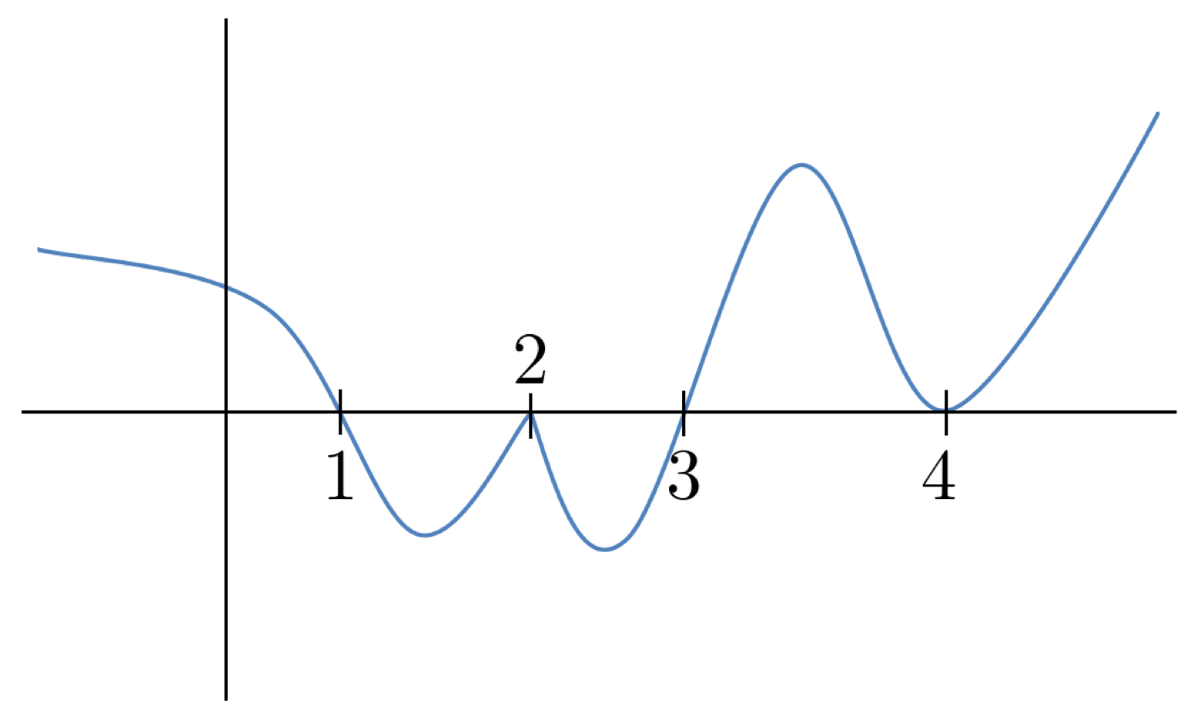
\includegraphics[width=0.5\textwidth]{ejer-a}
    \item Gr\'afica de la derivada de $f$.\\
        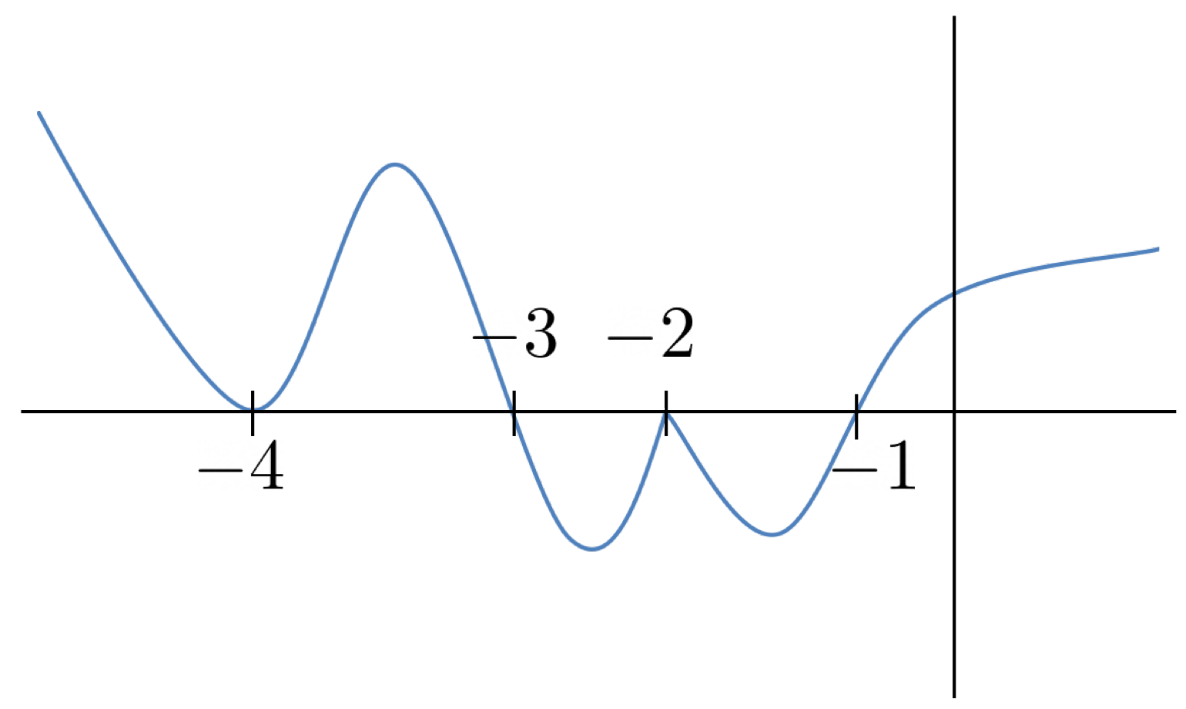
\includegraphics[width=0.5\textwidth]{ejer-b}
    \item Gr\'afica de la derivada de $f$.\\
        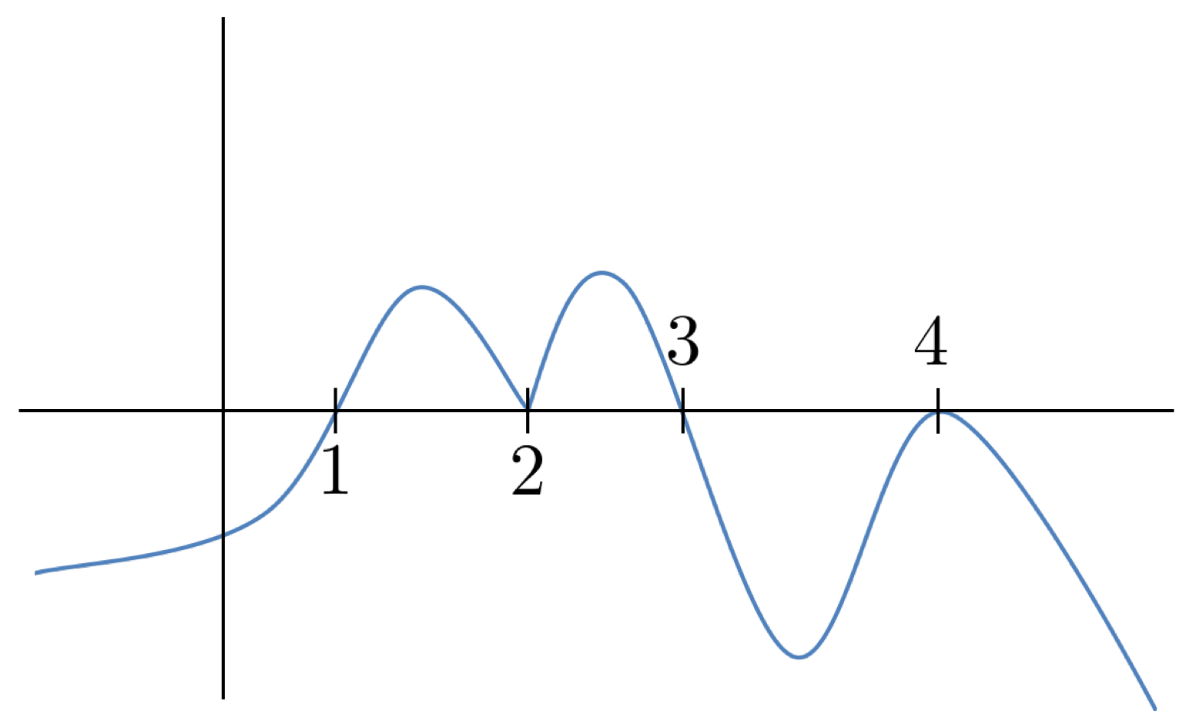
\includegraphics[width=0.5\textwidth]{ejer-c}
    \item Gr\'afica de la derivada de $f$.\\
        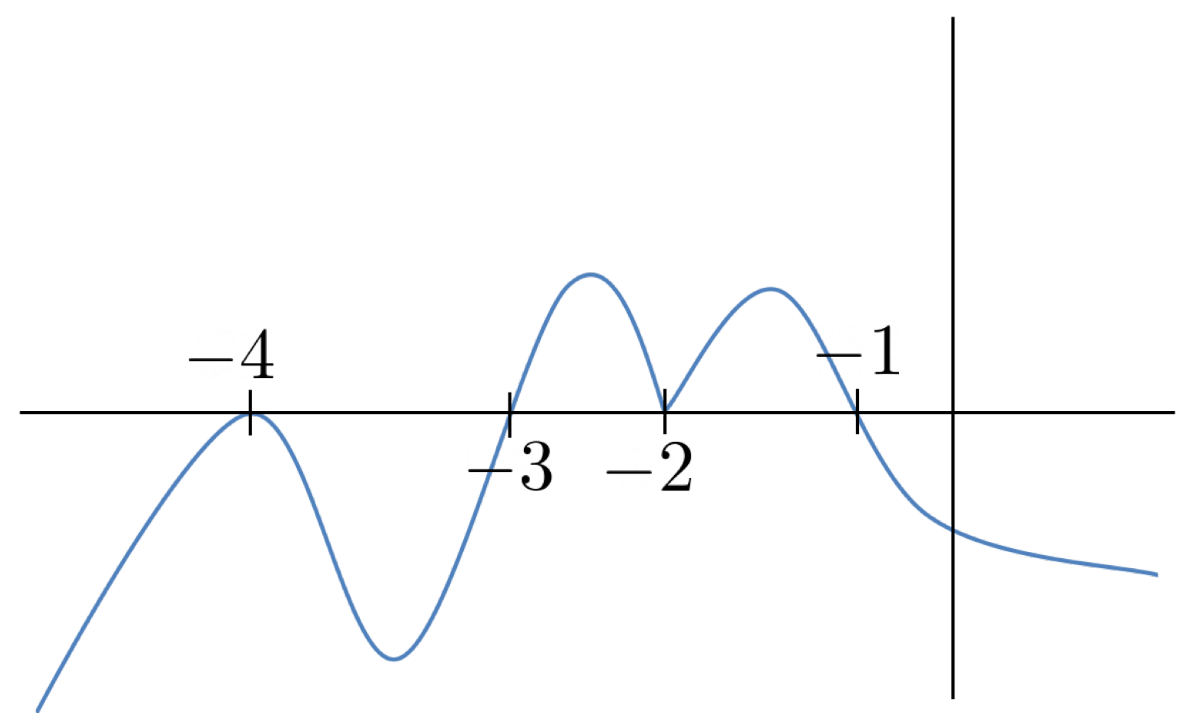
\includegraphics[width=0.5\textwidth]{ejer-d}
\end{enumerate}

%EJERCICIO 16 ----------------------------------------------------------------------------------
16. Utiliza los resultados sobre el significado de la derivada para esbozar la gr\'afica de las siguientes funciones (aplicar criterios de la primera y la segunda derivada).

\begin{enumerate}[\hspace{9px} a)]
    \item \(f(x)=x+\displaystyle\frac{1}{x}\)
    \item \(f(x)=x+\displaystyle\frac{3}{x^2}\)
    \item \(f(x)=\displaystyle\frac{x^2}{x^2-1}\)
    \item \(f(x)=\displaystyle\frac{1}{x^2+1}\)
\end{enumerate}

%EJERCICIO 17 ----------------------------------------------------------------------------------
17. Mostrar que:

\begin{enumerate}[\hspace{9px} a)]
    \item La suma de un n\'umero real positvio y su rec\'iproco es por lo menos 2.
    \item Entre todos los rect\'angulos de igual per\'imetro, el de mayor \'area es el cuadrado.
    \item Entre todos los rect\'angulos con la misma \'area, el cuadrado es el de per\'imetro m\'inimo.
    \item Entre todos los rect\'angulos que pueden inscribirse en una circunferencia, el cuadrado es el de \'area m\'axima.
    \item La raz\'on de variac\'on del volumen de una esfera rexpecto a su radio, es igual a su \'area.
\end{enumerate}

%EJERCICIO 18 ----------------------------------------------------------------------------------
18. Encuentre el punto para el cual:

\begin{enumerate}[\hspace{9px} a)]
    \item La recta tangente a la par\'abola \(f(x)=x^2-7x+3\), es paralela a la recta \(5x+3y-3=0\)
    \item La recta tangente a la par\'abola \(f(x)=x^2-7x+3\), es paralela a la recta \(3x-y-4=0\)
    \item La recta tangente a la pa\'rabola \(f(x)=x^2-7x+3\), es paralela a la recta \(2x+3y-3=0\)
\end{enumerate}

\vfill

\textbf{F\'ormula cuadratica:}
\begin{proof}
\begin{align*}
    ax^2+bx+c&=0\\
    (4a)(ax^2+bx+c)&=0(4a) \quad &&\text{Por el teorema $a=b \iff ac=bc$.}\\
    (4a)(ax^2+bx+c)&=0 &&\text{Por el teorema $0a=0$.}\\
    (4a)(ax^2)+(4a)(bx)+(4a)(c)&=0 &&\text{Por el axioma de la distributividad.}\\
    4a^2x^2+4abx+4ac&=0 &&\text{Operando.}\\
    4a^2x^2+4abx+4ac-4ac+b^2&=0+b^2-4ac &&\text{Por el teorema $a=b \iff a+c=b+c$.}\\
    4a^2x^2+4abx+0+b^2&=0+b^2-4ac &&\text{Por el axioma del inverso de la suma.}\\
    4a^2x^2+4abx+b^2&=b^2-4ac &&\text{Por el axioma del neutro de la suma.}\\
    (2ax+b)^2&=b^2-4ac &&\text{Por el teorema $(a+b)^2=a^2+2ab+b^2$.}\\
    2ax+b&=\pm \sqrt{b^2-4ac} &&\text{Sacando raiz cuadrada a ambos lados.}\\
    2ax+b-b&=-b \pm \sqrt{b^2-4ac} &&\text{Por el teorema $a=b \iff a+c=b+c$.}\\
    2ax+0&=-b \pm \sqrt{b^2-4ac} &&\text{Por el axioma del inverso de la suma.}\\
    2ax&=-b \pm \sqrt{b^2-4ac} &&\text{Por el axioma del neutro de la suma.}\\
    \frac{2ax}{2a}&=\frac{-b\pm \sqrt{b^2-4ac}}{2a} &&\text{Por el teorema $a=b \iff ac=bc$.}\\
    1x&=\frac{-b\pm \sqrt{b^2-4ac}}{2a} &&\text{Por el axioma del inverso de la multiplicación.}\\
    x&=\frac{-b\pm \sqrt{b^2-4ac}}{2a} &&\text{Por el axioma del neutro de la multiplicación.}
\end{align*}
\end{proof}

\end{document}
